\documentclass[10pt,a4paper]{book}
\usepackage{bm}
\usepackage{systeme}
\usepackage{enumitem}
\usepackage{hyperref}
\usepackage[utf8]{inputenc}
\usepackage[english]{babel}
\usepackage{hyperref}
\usepackage{tikz-cd}

\usepackage{amsmath}
\usepackage{amsthm}
\usepackage{amsfonts}
\usepackage{amssymb}


\newtheorem{thm}{Theorem}
\newtheorem{prop}[thm]{Proposition}
\newtheorem*{prop*}{Proposition}
\newtheorem{lem}[thm]{Lemma}
\newtheorem*{lem*}{Lemma}
\newtheorem{cor}[thm]{Corollary}
\newtheorem{rmk}[thm]{Remark}

\newcommand{\on}{\operatorname}
\newcommand{\s}{\on{Spec}}
\newcommand{\p}{\on{Proj}}
\newcommand{\mf}{\mathfrak}
\newcommand{\mc}{\mathcal}
\title{Notes from reading "Introduction to Toric Varieties" by Fulton}
\begin{document}
\maketitle
\chapter{Definitions and examples}
\section{Motivating Example}
Let $X\subseteq \mathbb{A}^3_\mathbb{C}$ be given by $y^3-xz=0$. Denote its coordinate ring by $R=\mathbb{C}[x,y,z]/(y^3-xz)$ and consider the action of $(\mathbb{C}^*)^2$ on $X$ given by:
\[
(t_1,t_2)\cdot (x,y,z) = (t_1^2t_2^3x, t_1t_2y, t_1z).
\]
We have an induced action of $(\mathbb{C}^*)^2$ on the coordinate ring $R$ given by 
\[
(t\cdot f)(p) = f(t\cdot p).
\]
Let $M =\{\chi\colon (\mathbb{C}^*)^2\to \mathbb{C}^*\}$ be the lattice of characters of $(\mathbb{C}^*)^2$. Recall that this group is isomorphic with $\mathbb{Z}^2$, $u\in \mathbb{Z}^2$ corresponding to $\chi^{u}\colon t\mapsto t^u$. Given $\chi^u\in M$, define $R_{u} = \{f\in R | t\cdot f = \chi^u(t)\cdot f\}$.
The class in $R$ of every monomial in $\mathbb{C}[x,y,z]$ can be written uniquely in the form $x^ay^bz^c$ with $b\in\{0,1,2\}$. We have $t_1^mt_2^n\cdot x^ay^bz^c = t_1^{m(2a+b+c)}t_2^{n(3a+b)}x^ay^bz^c$. Therefore, $x^ay^bz^c \in R_{u}$ if and only if $u = (2a+b+c, 3a+b)$. 
Let $u=(i,j)$. We search for a solution of the following system:
\[
\systeme*{2a+b+c = i, 3a+b = j, b\in\{\text{0,1,2}\},a\geq 0, c\geq 0}
\]
For every $(i,j)$ there is at most one solution, so $R=\bigoplus_{u\in \mathbb{Z}^2}R_u$ decomposes $R$ into one or zero dimensional subrepresentations of $(\mathbb{C}^*)^2$. We will find those $u=(i,j)$ for which $R_u$ is non-zero. We need to have $j\geq 0$ and then $a,b$ are uniquely determined. Therefore, if $j\geq 0$ then a solution exists if and only if $i-2a-b\geq 0$. This is equivalent to $3i-6a-3b\geq 0$. We can rewrite this as $3i \geq 2j+b$ which is equivalent to $3i\geq 2j$ since $2j+b = 6a+3b$ is divisible by 3 and $b\in\{0,1,2\}$. 

Therefore, for every $u\in \mathbb{Z}^2$ we have $\on{dim}_\mathbb{C} R_u \in \{0, 1\}$ and those $u$ for which $\on{dim}_\mathbb{C} R_u = 1$ are the lattice points of the cone below (cones will be formally defined in the next section).
\clearpage
\begin{figure}[h]
\centering
  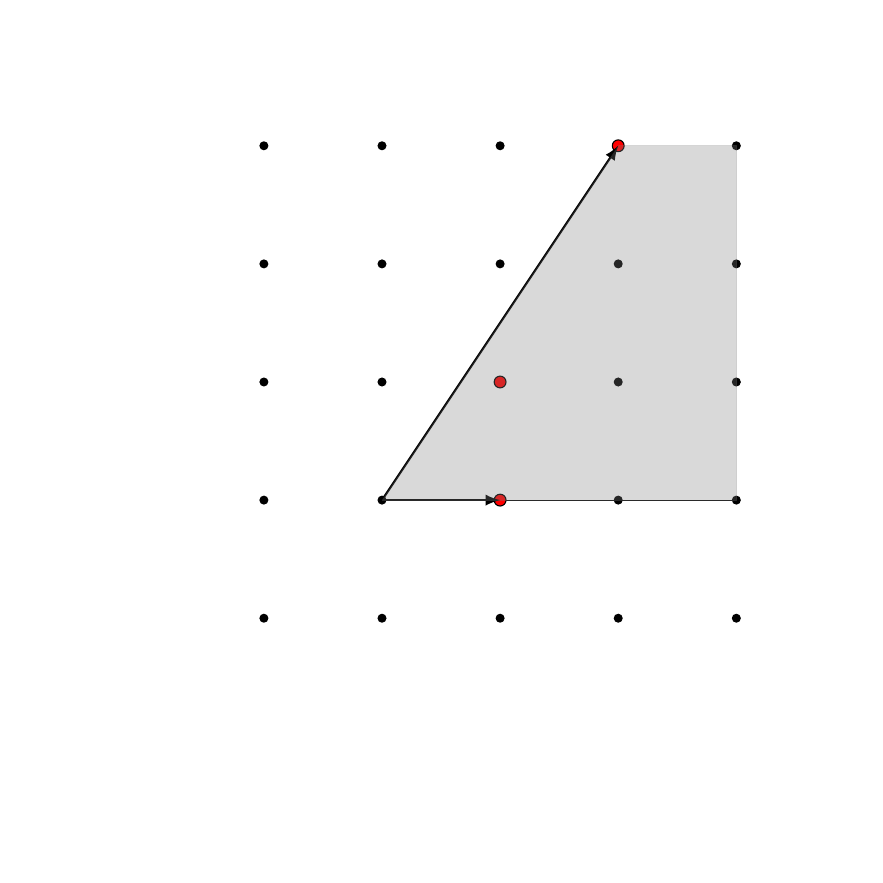
\begin{tikzpicture}[scale=1.50]
    \coordinate (Origin)   at (0,0);
    \coordinate (XAxisMin) at (-1,0);
    \coordinate (XAxisMax) at (3,0);
    \coordinate (YAxisMin) at (0,-1);
    \coordinate (YAxisMax) at (0,3);
   % \draw [thin, black,-latex] (XAxisMin) -- (XAxisMax);% Draw x axis
   % \draw [thin, black,-latex] (YAxisMin) -- (YAxisMax);% Draw y axis
	
    \clip (-3,-3) rectangle (4cm,4cm); % Clips the picture...
    \coordinate (Bone) at (1,0);
    \coordinate (Btwo) at (1,1);
    \coordinate (Bthree) at (2,3);         
    \foreach \x in {-1,...,3}{% Two indices running over each
      \foreach \y in {-1,...,3}{% node on the grid we have drawn 
        \node[draw,circle,inner sep=1pt,fill] at (\x,\y) {};
            % Places a dot at those points
      }
    }
	\draw [, black] (Origin) -- (3,0);
    \draw [, black] (Origin) -- (2,3);
	
	\draw[color=black, fill=red]   (1,0) circle (.05);
	\draw[color=black, fill=red]   (1,1) circle (.05);
	\draw[color=black, fill=red]   (2,3) circle (.05);
	
	
	\draw [thick,-latex,black] (Origin)
        -- (Bone) node [above] {};
    \draw [thick,-latex, black] (Origin)
    	-- (Bthree) node [above] {};
    
    \filldraw[fill=gray, fill opacity=0.3, draw=gray, draw opacity = 0.3] (0,0)--(3,0)--(3,3)--(2,3);
  \end{tikzpicture}
  \label{figure:fan of A^2}
\end{figure}
 Denote this cone by $\sigma^\vee$ and define the corresponding semigroup algebra $\mathbb{C}[\sigma^\vee \cap M] = \bigoplus_{u\in \sigma^\vee\cap M}\mathbb{C}\cdot \chi^u$ with multiplication induced by $\chi^u\cdot \chi^v = \chi^{u+v}$. Since $\sigma^\vee \cap M$ is generated as a semigroup by $(1,0), (1,1), (2,3)$, $\mathbb{C}[\sigma^\vee \cap M]$ is generated as a $\mathbb{C}$-algebra by $\chi^{(1,0)}$, $\chi^{(1,1)}$ and $\chi^{(2,3)}$. Moreover, the generators of the semigroup $\sigma^\vee \cap M$ satisfy a relation $3\cdot(1,1) = (1,0) + (2,3)$, therefore we have an isomorphism $\mathbb{C}[\sigma^\vee \cap M] \to R$ given by $\chi^{(1,0)}\mapsto x$, $\chi^{(1,1)}\mapsto y$ and $\chi^{(2,3)}\mapsto z$. 

\section{Convex polyhedral cones}
Let $V$ be the vector space $N_\mathbb{R}$, with dual space $V^* = M_\mathbb{R}$. A \textit{convex polyhedral cone} is a set 
\[
\sigma = \{r_1v_1+...+r_sv_s\in V: r_i\geq 0\}
\]
generated by any finite set of vectors $v_1,..., v_s \in V$. Such vectors, or sometimes the corresponding rays consisting of positive multiples of some $v_i$ are called \textit{generators} for the cone $\sigma$.


The \textit{dimension} $\on{dim}(\sigma)$ of $\sigma$ is the dimension of the linear space $\mathbb{R}\cdot \sigma = \sigma  + (-\sigma)$ spanned by $\sigma$. The \textit{dual} $\sigma^\vee$ of any set $\sigma$ is the set of equations of supporting hyperplanes, i.e.,
\[
\sigma^\vee = \{u\in V^*: \langle u,v \rangle \geq 0 \text{ for all }v\in \sigma\}.
\]

Everything is based on the following fundamental fact from the theory of convex sets.

\smallskip
\noindent (*) If  $\sigma$ is a convex polyhedral cone and  $v_0\notin \sigma$, then there is some  $u_0 \in \sigma^\vee$ with $\langle u_0, v_0 \rangle < 0.$
\smallskip

We list some consequences of (*). Since the proofs given in Fulton's text are easy to follow we do not replicate them here.
A direct translation of (*) is the duality theorem:

\smallskip
\noindent (1) $(\sigma^\vee)^\vee = \sigma.$
\smallskip

A \textit{face} $\tau$, of $\sigma$ is the intersection of $\sigma$ with any supporting hyperplane: $\tau= \sigma\cap u^\perp =\{v\in \sigma :\langle u, v \rangle = 0\}$ for some $u$ in $\sigma^\vee$. A cone is regarded as a face of itself, while others are called \textit{proper} faces. Note that any linear subspace of a cone is contained in every face of the cone,

\smallskip
\noindent (2) Any face is also a convex polyhedral cone. 
\smallskip

\smallskip
\noindent (3) Any intersection of faces is also a face.
\smallskip

\smallskip
\noindent (4) Any face of a face is a face.
\smallskip

A \textit{facet} is a face of codimension one.

\smallskip
\noindent (5) Any proper face is contained in some facet.
\smallskip

\smallskip
\noindent (6) Any proper face is the intersection of all facets containing it.
\smallskip

\smallskip
\noindent (7) The topological boundary of a cone that spans $V$ is the union of its proper faces (or facets).
\medskip

When $\sigma$ spans $V$ and $\tau$ is a facet of $\sigma$, there is a $u\in \sigma^\vee$, unique up to multiplication by a positive scalar, with $\tau= \sigma\cap u^\perp$. Such a vector, which we denote by $u_\tau$ is an equation for the hyperplane spanned by $\tau$.

\medskip
\noindent (8) If $\sigma$ spans $V$ and $\sigma \neq V$, then $\sigma$ is the intersection of the half-spaces $H_\tau = \{v\in V: \langle u_\tau, v \rangle \geq 0\}$, as $\tau$ ranges over the facets of $\sigma$.
\medskip

From (8) we deduce the fact known as Farkas' Theorem:

\medskip 
\noindent (9) The dual of a convex polyhedral cone is a convex polyhedral cone.
\medskip


This shows that polyhedral cones can also be given a dual definition as the intersection of half-spaces: for generators $u_1,...,u_t$ of $\sigma^\vee$,
\[
\sigma = \{v\in V: \langle u_1, v\rangle \geq 0, ..., \langle u_t, v\rangle \geq 0 \}.
\]
If we now suppose $\sigma$ is \textit{rational}, meaning that its generators can be taken from $N$, then $\sigma^\vee$ is also rational.

\begin{prop}[Gordan's Lemma] If $\sigma$ is a rational convex polyhedral cone, then $S_\sigma = \sigma^\vee \cap M$ is a finitely generated semigroup.
\end{prop}

It is often necessary to find a point in the \textit{relative interior} of a cone $\sigma$, i.e., in the topological interior of $\sigma$ in the space $\mathbb{R}\cdot \sigma$ spanned by $\sigma$. This is achieved by taking any positive combination of $\on{dim}(\sigma)$ linearly independent vectors among the generators of $\sigma$. In particular, if $\sigma$ is rational, we can find such points in the lattice.

\medskip
\noindent (10) If $\tau$ is a face of $\sigma$, then $\sigma^\vee \cap \tau^\perp$ is a face of $\sigma^\vee$, with $\on{dim}(\tau)+\on{dim}(\sigma^\vee \cap \tau^\perp) = n = \on{dim}(V).$ This sets up a one-to-one order-reversing correspondence between the faces of $\sigma$ and the faces of $\sigma^\vee$. The smallest face of $\sigma$ is $\sigma\cap (-\sigma)$.
\medskip

\medskip
\noindent (11) If $u\in \sigma^\vee$, and $\tau = \sigma\cap \tau^\perp$, then $\tau^\vee = \sigma^\vee + \mathbb{R}_{\geq 0}\cdot (-u)$.
\medskip

\begin{prop} Let $\sigma$ be a rational convex polyhedral cone, and let $u$ be in $S_\sigma=\sigma^\vee\cap  M$. Then $\tau = \sigma\cap u^\perp$ is a rational convex polyhedral cone. All faces of $\sigma$ have this form, and 
\[
S_\tau = S_\sigma + \mathbb{Z}_{\geq 0}\cdot(-u).
\]
\end{prop}

Finally, we need the following strengthening of (*), known as a \textit{Separation Lemma}, that separates convex sets by a hyperplane:

\medskip
\noindent (12) If $\sigma$ and $\sigma'$ are convex polyhedral cones whose intersection $\tau$ is a face of each, then there is a $u$ in $\sigma^\vee \cap (-\sigma')^\vee$ with
\[
\tau = \sigma \cap u^\perp  = \sigma'\cap u^\perp.
\]
\medskip


\begin{prop} If $\sigma$ and $\sigma'$ are rational convex polyhedral cones whose intersection $\tau$ is a face of each, then
\[
S_\tau = S_\sigma + S_{\sigma'}.
\]
\end{prop}	

\medskip
\noindent (13) For a convex polyhedral cone $\sigma$, the following conditions are equivalent:
\begin{itemize}
\item[(i)] $\sigma\cap (-\sigma) = \{0\}$;
\item[(ii)] $\sigma$ contains no nonzero linear subspace;
\item[(iii)] there is a $u$ in $\sigma^\vee$ with $\sigma\cap u^\perp = \{0\}$;
\item[(iv)] $\sigma^\vee$ spans $V^*.$ 
\end{itemize}
\medskip

A cone is called \textit{strongly convex} if it satisfies the conditions of (13). Any cone is generated by some minimal set of generators. If the cone is strongly convex, then the rays generated by a minimal set of generators are exactly the one-dimensional faces of $\sigma$ (as seen by applying (*) to any generator that is not in the cone generated by the others); in particular, these minimal generators are unique up to multiplication by positive scalars.

Since we are mainly concerned with these cones, we will often say "$\sigma$ is a cone in $N$" to mean that $\sigma$ is a strongly convex rational polyhedral cone in $N_\mathbb{R}$. We will sometimes write "$\tau \prec \sigma$" or "$\sigma \succ \tau$" to mean that $\tau$ is a face of $\sigma$. A cone is called \textit{simplicial}, or a \textit{simplex}, if it is generated by linearly independent generators.

\section{Affine toric varieties}
Let $R$ be a ring. We work in the category of $R$-schemes so affine space, multiplicative group, products, etc.  are all over $R$.
When $\sigma$ is a strongly convex rational polyhedral cone, we have seen that $S_\sigma = \sigma^\vee \cap M$ is a finitely generated semigroup. Any additive semigroup $S$ determines a "group ring" $R[S]$, which is a commutative $R$-algebra. As an $R$-module it has a basis $\chi^u$, as $u$ varies over $S$, with multiplication determined by the addition in $S$:
\[
\chi^u\cdot \chi^{u'} = \chi^{u+u'}.
\]
The unit $1$ is $\chi^0$. Generators $\{u_i\}$ for the semigroup $S$ determine generators $\{\chi^{u_i}$\} for the $R$-algebra $R[S]$. 

Any finitely generated commutative $R$-algebra $A$ determines an affine scheme of finite type over $R$, which we denote by $\s (A)$. We review this construction and its related notation. If generators of $A$ are chosen, this presents $A$ as $R[X_1,...,X_m]/I$, where $I$ is an ideal;
then $\s A$ can be identified with the subscheme $V(I)$ of affine space $\mathbb{A}^m$. In our applications, $A$ will be a domain, so $\s (A)$ will be an integral scheme. Although $\s (A)$ officially includes all prime ideals of $A$, when we speak of a \textit{point} of $\s (A)$ we will mean an $R$-point, i.e. a homomorphism of $R$-schemes $\s (R) \to \s (A)$, unless we specify otherwise. Any homomorphism $A \to B$ of $R$-algebras determines a morphism $\s (B)\to \s (A)$ of
$R$-schemes. In particular, $R$-points correspond to $R$-algebra homomorphisms from $A$ to $R$. If $X = \s (A)$, for each nonzero element $f \in A$ the principal open subset
\[
X_f = \s(A_f) \subset X = \s (A)
\]
corresponds to the localization homomorphism $A\to A_f$. 

For $A = R[S]$ constructed from a semigroup, the points are easy to describe: they correspond to homomorphisms of semigroups from $S$ to $R$, where $R$ is regarded as an abelian semigroup via
multiplication:
\[
(\s (R[S]))(R) = \on{Hom}_{sg}(S, R).
\]
Indeed, this follows from the adjunction $R[-] \dashv G$ where $G$ is the forgetful functor from the category of $R$-algebras to the category of monoids mapping an $R$-algebra to the underlying multiplicative monoid.

When $S_\sigma$ arises from a strongly convex rational polyhedral cone, we set $A_\sigma = R[S_\sigma]$, and $U_\sigma = \s (R[S_\sigma]) = \s (A_\sigma)$, the corresponding \textit{affine toric scheme}. All of these semigroups will be sub-semigroups of the group $M = S_{\{0\}}$. If $e_1,..., e_n$ is a basis for $N$, and $e_1^*,..., e_n^*$ is the dual basis of $M$, write 
\[
X_i = \chi^{e_i^*} \in R[M].
\]
As a semigroup, $M$ has generators $\pm e_1^*, ..., \pm e_n^*$, so
\[
R[M] = R[X_1,X_1^{-1},X_2,X_2^{-1},... ,X_n, X_n^{-1}] = R[X_1,...,X_n]_{X_1\cdot... \cdot X_n},
\]
which is the ring of \textit{Laurent polynomials} in $n$ variables. So
\[
U_{\{0\}} = \s (R[M])\cong \mathbb{G}_m^n
\]
is an affine algebraic torus. All of our semigroups $S$ will be sub-semigroups of a lattice $M$, so $R[S]$ will be a subalgebra of $R[M]$; in particular, $R[S]$ will be a domain if $R$ is an integral domain. When a basis for $M$ is chosen as above, we usually write elements of $R[S]$ as Laurent polynomials in the corresponding variables $X_i$. Note that all of these algebras are generated by \textit{monomials} in the variables $X_i$.

The torus $T = T_N$ corresponding to $M$ or $N$ can be written intrinsically:
\[
T_N(R) = (\s (R[M]))(R) = \on{Hom}_{group}(M,R^*) = N\otimes_\mathbb{Z}R^*.
\]
The above uses the adjunction $R[-]\dashv [-]^*$ where $[-]^*$ is the functor from the category of $R$-algebras to the category of groups mapping underlying ring to its group of invertible elements.

For a basic example, let $\sigma$ be the cone with generators $e_1,..., e_k$ for some $k$, $1 \leq k \leq n$. Then
\[
S_\sigma = \mathbb{Z}_{\geq 0}\cdot e_1^* + \mathbb{Z}_{\geq 0}\cdot e_2^* + ... + \mathbb{Z}_{\geq 0}\cdot e_k^* + \mathbb{Z}\cdot e_{k+1}^* + ... + \mathbb{Z}\cdot e_n^*.
\]
Hence $A_\sigma = R[X_1, X_2, ..., X_k, X_{k+1}, X_{k+1}^{-1}, ..., X_n, X_n^{-1}]$, and
\[
U_\sigma = \mathbb{A}^k \times \mathbb{G}_m^{n-k}.
\]
It follows from this example that if $\sigma$ is generated by $k$ elements that can be completed to a basis for $N$, then $U_\sigma$ is a product of affine $k$-space and an algebraic torus of rank $(n-k)$. In particular, such affine toric schemes are smooth over $R$.

Next we look at a singular example. Let $N$ be a lattice of rank $3$, and let $\sigma$ be the cone generated by four vectors $v_1, v_2, v_3,$ and $v_4$ that generate $N$ and satisfy $v_1 + v_3 = v_2 + v_4$. The scheme $U_\sigma$ is a "cone over a quadric surface", a scheme met frequently when
singularities are studied. If we take $N = \mathbb{Z}^3$ and $v_i = e_i$ for $i = 1, 2, 3,$ so $v_4 = e_1 + e_3 - e_2,$ then $S_\sigma$ is generated by $e_1^*, e_3^*, e_1^*+e_2^*$, and $e_2^*+e_3^*$, so
\[
A_\sigma = R[X_1,X_3, X_1X_2, X_2X_3] = R[W,X,Y,Z]/(WZ-XY).
\]

A homomorphism of semigroups $S \to S'$ determines a homomorphism \linebreak $R[S] \to R[S']$ of algebras, hence a morphism $\s(R[S']) \to \s(R[S])$ of affine $R$-schemes. In particular, if $\tau$  is contained in $\sigma$, then $S_\sigma$ is a sub-semigroup of $S_\tau$, corresponding to
a morphism $U_\tau \to U_\sigma$. For example, the torus $T_N = U_{\{0\}}$ maps to all
of the affine toric schemes $U_\sigma$ that come from cones $\sigma$ in $N$.

\begin{lem*} If $\tau$ is a face of $\sigma$, then the map $U_\tau \to U_\sigma$ embeds $U_\tau$ as a principal open subset of $U_\sigma$.
\end{lem*}
\begin{proof}
By Proposition 2 in \S 1.2, there is a $u\in S_\sigma$ with $\tau = \sigma \cap u^\perp$ and
\[
S_\tau = S_\sigma + \mathbb{Z}_{\geq 0}\cdot(-u).
\]
This implies immediately that each basis element for $R[S_\tau]$ can be written in the form $\chi^{w-pu} = \chi^w/(\chi^u)^p$ for $w\in S_\sigma$. Hence
\[
A_\tau = (A_\sigma)_{\chi^u},
\]
which is the algebraic version of the required assertion.
\end{proof}

More generally, if $\varphi\colon N' \to N$ is a homomorphism of lattices such that $\varphi_\mathbb{R}$ maps a (rational strongly convex polyhedral) cone $\sigma'$ in $N'$ into a cone $\sigma$ in $N$, then the dual $\varphi^\vee \colon M \to M'$ maps $S_\sigma$ to $S_{\sigma'},$ determining a homomorphism $A_\sigma \to A_{\sigma'}$, and hence a morphism $U_{\sigma'}\to U_\sigma.$

The semigroups $S_\sigma$ arising from cones are special in several respects. First, it follows from the definition that $S_\sigma$ is \textit{saturated}, i.e., if $p\cdot u$ is in $S_\sigma$ for some positive integer $p$, then $u$ is in $S_\sigma$. In addition, the fact that $\sigma$ is strongly convex implies that $\sigma^\vee$ spans $M_\mathbb{R}$, so $S_\sigma$ generates $M$ as a group, i.e.,
\[
M = S_\sigma + (-S_\sigma).
\]

If $\sigma$ is a cone in $N$, the torus $T_N$ acts on $U_\sigma$,
\[
T_N \times U_\sigma \to U_\sigma,
\]
as follows. A point $t\in T_N(R)$ can be identified with a map $M\to R^*$ of groups, and a point $x\in U_\sigma(R)$ with a map $S_\sigma \to R$ of semigroups; the product $t\cdot x$ is the map of semigroups $S_\sigma \to R$ given by
\[
u \mapsto  t(u)x(u).
\]
The dual map on algebras, $R[S_\sigma] \to R[S_\sigma]\otimes R[M]$, is given by mapping $\chi^u$ to $\chi^u\otimes \chi^u$ for $u\in S_\sigma$. When $\sigma =\{0\}$, this is the usual product in the algebraic group $T_N$. These maps are compatible with inclusions
of open subsets corresponding to faces of $\sigma$. In particular, they extend the action of $T_N$ on itself.


To say it differently, the multiplication in $\mathbb{G}_m^n$ is known to correspond to the homomorphism $m^\# \colon R[M] \to R[M]\otimes R[M]$ given by $\chi^u\mapsto \chi^u\otimes \chi^u$. Therefore, if we define $\mu^\#\colon R[S_\sigma]\to R[M]\otimes R[S_\sigma]$ by $\chi^u\mapsto \chi^u\otimes \chi^u$ the following diagram is commutative:
\begin{center}
\begin{tikzcd}
R[S_\sigma] \arrow[r, "\mu^\#"] \arrow[d, hook] & R[M]\otimes R[S_\sigma] \arrow[d, hook]\\
R[M] \arrow[r, "m^\#"] & R[M]\otimes R[M].
\end{tikzcd}
\end{center}
so that $\mu\colon T_N\times U_\sigma \to U_\sigma$ extends $m\colon T_N\times T_N \to T_N$. In order to check that this is an action we should check that the following diagrams are commutative:

\begin{center}
\begin{tikzcd}
T_N\times T_N \times U_\sigma \arrow[r, "\on{id}\times \mu"] \arrow[d, "m\times \on{id}"] & T_N \times U_\sigma \arrow[d, "\mu"]\\
T_N\times U_\sigma \arrow[r, "\mu"] & U_\sigma
\end{tikzcd} \begin{tikzcd}
\s R \times U_\sigma \arrow[r, "e\times \on{id}"] \arrow[dr, "\cong"'] & T_N \times U_\sigma \arrow[d, "\mu"]\\
& U_\sigma
\end{tikzcd}
\end{center}
This can be verified directly on algebras using the fact that $e:\s R \to T_N$ corresponds to $R[M]\to R$ given by $\chi^u\mapsto 1$ for all $u\in M$ and the isomorphism in the right diagram corresponds to the standard isomorphism $R[S_\sigma]\to R\otimes_R R[S_\sigma]$.



\chapter{Singularities and compactness}

\section{Local properties of toric varieties}
For any cone $\sigma$ in a lattice $N$, the corresponding affine scheme $U_\sigma$ has a distinguished point, which we denote by $x_\sigma$. This point in $U_\sigma$ is given by a map of semigroups
\[
S_\sigma = \sigma^\vee \cap M \to R,
\]
defined by the rule
\[
u \mapsto \begin{cases}
1 & \text{ if } u\in \sigma^\perp\\
0 & \text{ otherwise}.
\end{cases}
\]
Note that this is well defined since $\sigma^\perp$ is a face of $\sigma^\vee$, which implies
that the sum of two elements in $\sigma^\vee$ cannot be in $\sigma^\perp$ unless both are in $\sigma^\perp$.

\begin{prop*} An affine toric scheme $U_\sigma$ is smooth over $\s (R)$ if and only if $\sigma$ is generated by part of a basis for the lattice $N$, in which case
\[
U_\sigma \cong \mathbb{A}^k\times \mathbb{G}_m^{n-k} \text{, } k =\on{dim}(\sigma).
\]
\end{prop*}
\begin{proof}
It is enough to show that if $U_\sigma$ is smooth over $\s (R)$ then $\sigma$ is generated by part of a basis for the lattice $N$. Suppose to start that $\sigma$ spans $N_\mathbb{R}$, so $\sigma^\perp = \{0\}$. Assume that $U_\sigma$ is smooth over $R$ and let $\mf{n}$ be a maximal ideal of $R$ with $K=R/\mf{n}$. Take the base change:
\begin{center}
\begin{tikzcd}
U_\sigma \times_R K \arrow[r] \arrow[d, "\pi'"] & U_\sigma \arrow[d, "\pi"]\\
\s K \arrow[r] & \s R.
\end{tikzcd}
\end{center}
Note that $U_\sigma \times_R K$ is the affine toric variety associated with the cone $\sigma$ if we work in the category of $K$-schemes. Moreover, since $\pi$ is smooth, so is $\pi'$. Therefore, we may assume from the start that $U_\sigma$ is a variety over a field $K$. Then $\pi$ being smooth implies that $U_\sigma$ is a regular scheme. Consider the maximal ideal $\mf{m} = (\chi^u:u\in S_\sigma\setminus \{0\})$ of $A_\sigma = K[\sigma^\vee\cap M]$. The square $\mf{m}^2$ is generated by all $\chi^u$ for those $u$ that are sums of two elements of $S_\sigma\setminus \{0\}$. The cotangent space $\mf{m}/\mf{m}^2$ therefore has a basis of images of elements $\chi^u$ for
those $u$ in $S_\sigma \setminus \{0\}$ that are not the sums of two such vectors. For
example, the first elements in $M$ lying along the edges of $\sigma^\vee$ are vectors of this kind. Since $U_\sigma$ is regular, 
the cotangent space $\mf{m}/\mf{m}^2$ is $n$-dimensional, since $\on{dim}(U_\sigma) = \on{dim}(T_N) = n.$ This implies in particular that $\sigma^\vee$ cannot have more than $n$ edges, and that the
minimal generators along these edges must generate $S_\sigma$. Since $S_\sigma$ generates $M$ as a group, the minimal generators for $S_\sigma$ must be a basis for $M$. The dual $\sigma$ must therefore be generated by a basis for $N$. Hence $U_\sigma$ is isomorphic to affine space $\mathbb{A}^n_K$.

Consider now a general case when $\sigma$ has smaller dimension $k$. Let
\[
N_\sigma = \sigma\cap N + (-\sigma \cap N)
\]
be the sublattice of $N$ generated (as a subgroup) by $\sigma\cap N$. Since $\sigma$ is
saturated, $N_\sigma$ is also saturated, so the quotient group $N(\sigma) = N/N_\sigma$ is
also a lattice. We may choose a splitting and write
\[
N=N_\sigma \oplus N'' \text{, } \sigma =\sigma'\oplus \{0\},
\]
where $\sigma'$ is a cone in $N_\sigma$. Decomposing $M = M'\oplus M''$ dually, we
have $S_\sigma = ((\sigma')^\vee \cap M')\oplus M''$, so
\[
U_\sigma \cong U_{\sigma'}\times T_{N''} \cong U_{\sigma'}\times \mathbb{G}_m^{n-k}.
\]
As before, by taking a base change, we may assume that we work over a field $K$. Since $U_\sigma$ is smooth over $K$ and $U_{\sigma'}$,$T_{N''}$ are affine schemes of finite type over $K$, they must be both smooth.
Indeed, $\on{dim} U_\sigma = \on{dim}U_{\sigma'}+\on{dim}T_{N''}$ by \cite[Prop.~5.37]{gortz2010algebraic}. We may choose a presentation of $U_{\sigma'}$, $T_{N''}$ as subschemes of affine spaces and then the Jacobian corresponding to $U_\sigma$ is a block matrix with blocks corresponsing to Jacobians of $U_{\sigma'}$ and $T_{N''}$. Therefore, the preceding discussion applies: $\sigma'$ must be generated by a basis for $N_\sigma$.
\end{proof}

We therefore call a cone \textit{nonsingular} if it is generated by part of a basis for the lattice, and we call a fan \textit{nonsingular} (fan is defined in \S 1.4) if all of its cones
are nonsingular, i.e., if the corresponding toric scheme is smooth. Although a toric scheme may be singular, every toric scheme is normal if the base ring is an integrally closed domain:

\begin{prop*} If the base ring $R$ is integrally closed, then each ring $A_\sigma$ is integrally closed.
\end{prop*}
\begin{proof}
If $\sigma$ is generated by $v_1,...,v_r$, then $\sigma^\vee = \cap \tau_i^\vee$, where
$\tau_i$ is the ray generated by $v_i\in \sigma$, so $A_\sigma = \cap A_{\tau_i}$. We have seen that each $A_{\tau_i}$ is isomorphic to $R[X_1,X_2, X_2^{-1}, ..., X_n, X_n^{-1}]$, which is integrally closed (polynomial ring over a normal domain is a normal domain and localization of a normal domain is a normal domain), and the proposition follows from the fact that the intersection of integrally closed domains with common field of fractions is integrally closed.
\end{proof}


\bibliographystyle{unsrt}
\bibliography{biblio}
\end{document}